\section{Overview of MimbleWimble \& Grin}
\label{scn:grin_overview}

MimbleWimble \cite{Poelstra2016} is a blockchain protocol relying only on elliptic curve cryptography and promises to provide scalability, privacy and fungibility all at once.
Interestingly, MimbleWimble does not have any addresses or accounts and the amounts also are hidden using Pedersen commitments.
The simple design of MimbleWimble coupled with its privacy and scalability guarantees (which most existing blockchain implementations fail to address collectively) is what makes it popular for use in decentralized systems.
Grin \cite{GrinWebsite} and Beam \cite{BeamWebsite} are cryptocurrency systems which are powered by the MimbleWimble protocol.

\subsection{Outputs in Grin}

Amounts in MimbleWimble are hidden in Pedersen commitments known as \textit{outputs}.
An output containing amount $a \in \{0,1,\dots, 2^{64}-1\}$ is of the form\footnote{We use additive notation in this section only to be consistent with the original MimbleWimble protocol in \cite{Poelstra2016}.} $P = kG + aH$ where $r \in \Z_q$ and $G,H$ are generators of $\G$.
Note that the discrete log relation between $G$ and $H$ is assumed to be unknown.
The quantity $k$ is called as the \textit{blinding factor} and it serves as the secret key of output $P$.
Knowledge of $k$ implies ownership of the output.
At the time of creation of new outputs, they are accompanied by a range proof which proves that the amounts hidden in them lie in a finite range.

\subsection{Transactions in Grin}
A Grin transaction consists of some inputs which are being spent and some outputs in which the funds would be deposited.
Note that the inputs in a transaction are essentially outputs which were generated in some block in the past.
Grin transactions are of two types: (i) coinbase transactions, which transfer the block mining rewards to miners and (ii) regular transactions, which makes up for amount transfers in non-miners.
Coinbase transactions do not contain any inputs and typically have just one output known as \textit{coinbase} output.
A regular Mimblewimble transaction \cite{GrinDocOnGithub} includes the following:
\begin{enumerate}
    \item[(i)] A set of inputs, that reference and spend a set of previous outputs,
    \item[(ii)] A set of new outputs each with a range proof,
    \item[(iii)] An transaction fee,
    \item[(iv)] A Schnorr signature whose private key is computed by taking the excess amount (the sum of all output amounts plus the fee, minus the input amounts),
    \item[(v)] The public key published with the Schnorr signature is known as \textit{kernel excess} and is of the form $rG, \ r \in \Z_q$.
\end{enumerate}
We will refer to the collection of transaction fee, public key and signature as a \textit{kernel}.
Note that a transaction can easily be validated by determining that the kernel excess is a valid public key. 

\subsection{Transaction Aggregation}
Transactions in a Grin block are aggregated before the block is added to the blockchain to ensure unlinkability in inputs and outputs.
Consider the following example where we intend to aggregate two given regular transactions.
\begin{table}[h!]
  \centering
    \begin{tabular}{ | m{3cm} | m{2cm}| m{2cm} | m{2cm} | m{2cm} |} 
    \hline
                           & Inputs & Outputs & Excesses & Fee \\
    \hline
    Tx\#1         & $I_1, I_2$ & $O_1$ & $K_1$  & $f_1$ \\ 
    \hline
    Tx\#2         & $I_3$ & $O_2$ & $K_2$  & $f_2$ \\ 
    \hline
    \hline
    Aggregated Tx & $I_1, I_2, I_3$ & $O_1, O_2$ & $K_1, K_2$  & $f_1 + f_2$\\ 
    \hline
    \end{tabular}
  \caption{Example of Transaction Aggregation}
  \label{table:tx_agg}
\end{table}

\noindent
However, there is a slight issue here. 
It is possible to try all combinations of inputs and outputs to recover one of the transactions where the equality 
$$\sum (\text{Ouputs}) + \sum (\text{Fees})H - \sum (\text{Inputs}) = \text{Kernel excess}$$
satisfies. To mitigate this, the kernel excess is redefined from $rG$ to $(r-k_{\text{offset}})G$ where $r$ is the sum of output amounts plus fees minus input amounts and $k_{\text{offset}}$ is a scalar in $Z_q$.
Thus, The kernel offset $k_{\text{offset}}$ is thus a blinding factor that needs to be added to the excess value to ensure the commitments sum to zero as:
\begin{equation*}
  \sum (\text{Ouputs}) + \sum (\text{Fees})H - \sum (\text{Inputs}) = \text{Kernel excess} + k_{\text{offset}}G
\end{equation*}

Further, if in a same block, some outputs generated in a transaction are spent in the same block in another transaction, we can drain those outputs and inputs from the block as the structure of each transaction does not actually matter.
As long as the sum of inputs and outputs cancels off, removing matching outputs would not matter. 
This is known as \textit{cut-through}. 

Going a step further, all the blocks on the Grin blockchain can be considered as individual transactions. 
Thus, the outputs generated at block height $h_1$ which are spent as inputs in block $h_2$ also could be removed from the blockchain as they can be considered intermediate transactions by the same logic as above.
This significantly improves scalability of MimbleWimble-based blockchains.  

\subsection{Grin Blocks}
\label{scn:GrinOverview}

%Grin is an implementation of the MimbleWimble protocol and thus it does not have any addresses.
Let $\mathbb{G}$ be the secp256k1 elliptic curve group of order $n$.
In Grin, coins are stored in Pedersen commitments of the form $C = kG + aH$ where $k, a \in \mathbb{F}_n$ are scalars and $G, H \in \mathbb{G}$ are the generators of $\mathbb{G}$ with an unknown discrete logarithm with respect to each other.
%Also, the discrete logarithm relation between $G$ and $H$ is assumed to be unknown. Grin uses the elliptic curve group secp256k1.
The quantity $a$ is the amount stored in $C$ and $k$ is a randomly chosen scalar known as the blinding factor. 
A Grin block consists of the following:
\begin{enumerate}
  \item[(i)] A block header from which a scalar $k_{\text{off}} \in \mathbb{F}_n$ called the \textit{kernel offset} can be derived. The other header fields are not relevant to our discussion.
  \item[(ii)] A list of $L$ input commitments $I_1, I_2,\ldots,I_L$. This list is empty for blocks without regular transactions. Each input commitment refers to an output commitment in a previous block.
  \item[(iii)] A list of $M$ output commitments $O_1, O_2,\ldots,O_M$ where $M \ge 1$. Each output commitment is tagged as either a coinbase output or a regular transaction output. Each output commitment is also accompanied by a range proof to prove that it commits to an amount in the range $\{0,1,2, \dots,2^{64}-1\}$.  
  \item[(iv)] A list of $N$ \textit{transaction kernels} each of which contains a fee amount $f_i \in \mathbb{F}_n$ and a curve point $X_i \in \mathbb{G}$ called the \textit{kernel excess}. Each kernel also contains a Schnorr signature proving that $X_i$ is of the form $x_iG$ for some $x_i \in \mathbb{F}_n$. Each transaction kernel is also tagged either as a coinbase kernel or a regular transaction kernel.
\end{enumerate}

\begin{figure}[t]
  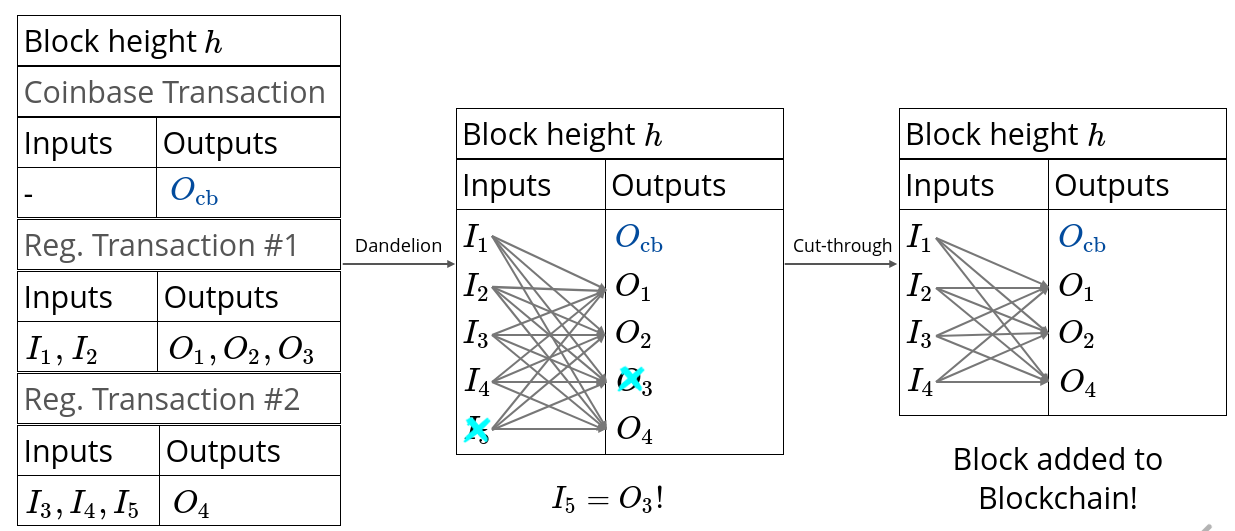
\includegraphics[width=0.92\textwidth]{Figures/block1.png}
  \centering
  \caption{A visual of the Dandelion protocol for transaction aggregation and the process of cut-through.
  Note that the coinbase outputs are denoted as $O_{\text{cb}}$ in blue colour.}
  \label{fig:dandelion}
\end{figure}

\begin{figure}[h!]
  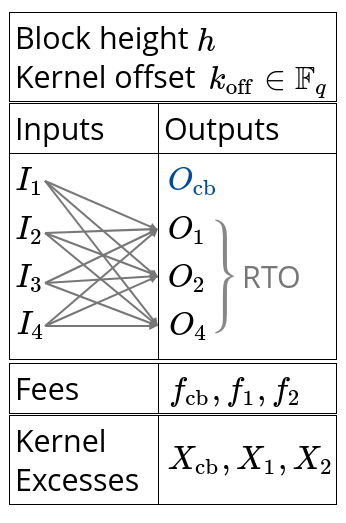
\includegraphics[width=0.27\textwidth]{Figures/block2.png}
  \centering
  \caption{Inclusion of kernels and fees in a Grin block. Note that the total number of transactions in a block are equal to the total number of kernels in a block.
  Also, $f_{\text{cb}} = 0$, the fees for coinbase transaction, for all Grin blocks.}
  \label{fig:kernels}
\end{figure}

% Each of these commitments refers to an output commitment in a previous block.An output is known as a \textit{coinbase} output if it is included by miners to store the mining reward and fees they earn
%during block mining. This transaction is known as \textit{coinbase} transaction.
%An output as a part of a regular transaction is known as \textit{transaction} output. 
%Each output is accompanied by a range proof to prove that it commits to an amount in the range $\{0,1,2, \dots,2^{64}-1\}$.  
%A Grin transaction consists of the following entities:
%\begin{enumerate}
%  \item[(i)] A vector of inputs serving as the sources of coins in the transaction. Each input is essentially an unspent output from some previous block.
%  \item[(ii)] A vector of outputs representing the destinations of coins in the transaction.
%  \item[(iii)] A vector of transaction kernels which are used in verification of transaction validity.
%\end{enumerate}
%A kernel is either a coinbase or a plain kernel according to the type of transaction.
%% A plain kernel is called as \textit{height-locked} kernel if the underlying transaction restricts its inclusion until a block at a specified height is mined.
%Each kernel contains the transaction fee and a \textit{kernel excess} which is a point on the curve of the form $xG$ where $x \in \mathbb{F}_n$.
%The kernel excess is accompanied by a Schnorr signature proving that it is of the form $xG$.
%% Transaction fee is included as a part of the kernel.
%
%A Grin block is characterized by a unique field called \textit{hash} which is SHA256 hash of its contents.
%% Each block contains the details of the Proof-of-Work used for mining.
%The inputs and outputs in a block are aggregated and we cannot distinguish between inputs and outputs of individual transactions.
%However, the total number of transactions in a block is equal to the number of kernels in that block.
%Suppose a block contains $L$ inputs $I_1, I_2, \dots, I_L$, $M$ outputs $O_1,O_2, \dots, O_M$
%and $N$ kernel excesses $X_1, X_2 \dots, X_N$ with individual fees $f_1, f_2 \dots, f_N$.
Refer to Figures \ref{fig:dandelion}, \ref{fig:kernels} for visual representation of a typical Grin block.
Let $\mathcal{I}_{\text{cb}} \subset \{1,2,\ldots,M\}$ be the set of indices corresponding to coinbase outputs and $\mathcal{I}_{\text{cb}}^c$ be the set of the remaining indices corresponding to RTOs. Let $\mathcal{I}_{\text{ck}} \subset \{1,2,\ldots,N\}$ be the set of indices corresponding to coinbase kernels and $\mathcal{I}_{\text{ck}}^c$ be the set of indices corresponding to regular transaction kernels. A valid block has to satisfy the following equations.
\begin{align}
  \sum_{i \in \mathcal{I}_{\text{cb}}} O_i - \left(\sum_{i=1}^{N}f_i\right)H - r H & = \sum_{i \in \mathcal{I}_{\text{ck}}} X_i,\\
  \sum_{i \in \mathcal{I}_{\text{cb}}^c} O_i + \left(\sum_{i=1}^{N}f_i\right)H - \sum_{i=1}^{L} I_i & = \sum_{i \in \mathcal{I}_{\text{ck}}^c} X_i + k_{\textnormal{off}}G.
  %\sum_{i=1}^{L} O_i + \left(\sum_{i=1}^{N}f_i\right)H - \sum_{i=1}^{M} I_i = \sum_{i=1}^{M} X_i + k_{\textnormal{off}}G
  \label{eqn:BlockValidity}
\end{align}
Here $r = 60\times 10^9$ is the block subsidy in nanogrin units.
As the right hand sides of both equations are commitments to the zero amount, the binding property of Pedersen commitments and the range proofs imply that
\begin{enumerate}
  \item[(i)] the total amount in the coinbase outputs of a block is $r + \sum_{i=1}^{N} f_i$ and
  \item [(ii)] the sum of the input amounts is equal to the sum of the transaction fees and RTO amounts.
\end{enumerate}
% The sum of coefficients of $H$ is zero in the above equation ensuring that no new coins are created.
%To see why (\ref{eqn:BlockValidity}) is enough to ensure validity of transactions, let
%$O_i = k_i^{\textnormal{out}}G + v_i^{\textnormal{out}}H$,
%$I_i = k_i^{\textnormal{in}}G + v_i^{\textnormal{in}}H$ and $X_i = x_iG$. Equation (\ref{eqn:BlockValidity}) holds only if the following hold
%\begin{align}
%  \sum_{i=1}^{M} v_i^{\textnormal{in}} &= \sum_{i=1}^{L} v_i^{\textnormal{out}} + \sum_{i=1}^{N}f_i \label{eqn:AmountEq} \\
%  \sum_{i=1}^{L} k_i^{\textnormal{out}} - \sum_{i=1}^{M} k_i^{\textnormal{in}} &= \sum_{i=1}^{N}x_i + k_{\textnormal{off}} \label{eqn:blindingFEq}
%\end{align}
%Equation (\ref{eqn:AmountEq}) implies that no new money was created and (\ref{eqn:blindingFEq}) implies that the coefficients of $G$ balance out.
%The reason for including $k_{\textnormal{off}}$ is to hide the relationship between the inputs and outputs in a block.
%If there were no kernel offset in a transaction, an adversary could attempt to deconstruct the individual transactions by trying combinations of inputs, outputs and kernels satisfying the transaction validity equation.
%
%A Grin block looks like a single transaction consisting of the aggregated inputs and outputs.
%If any output appears as an input in the same block, both of them are removed as they are not required for the block validation.
%Similarly, once an output is spent, it can be removed from the blockchain. 
%This process is known as \textit{cut-through} which improves scalability of Grin. 

